\chapter{Déploiement, Opérations et Sécurité}
\label{chap:deploiement}

\section{Stratégie de Conteneurisation Multi-Étapes (Docker)}

Pour assurer une portabilité totale du système et éliminer les disparités d'environnements, Perceptra est entièrement conteneurisé à l'aide d'un fichier \textbf{Dockerfile} multi-étapes (\textit{multi-stage build}).

Cette approche sépare la compilation des dépendances de la phase d'exécution finale, réduisant la taille de l'image de production et minimisant la surface d'attaque.

\begin{figure}[H]
\centering
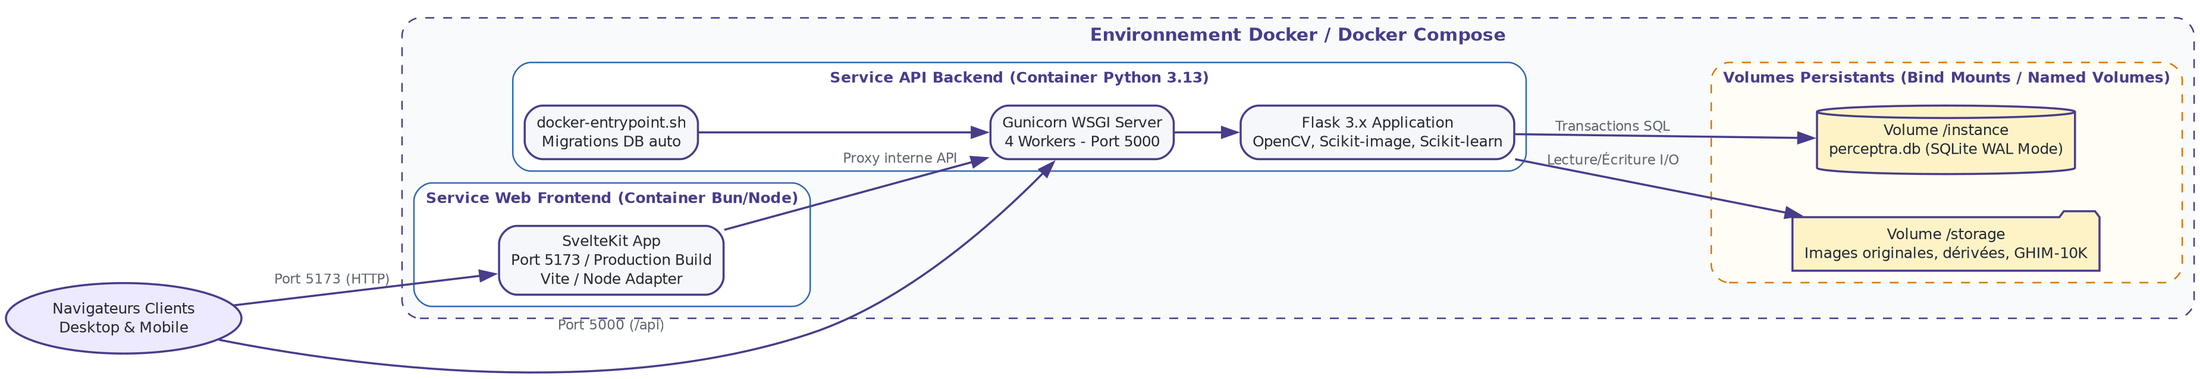
\includegraphics[width=0.78\textwidth]{images/10-deploiement-docker-infra.png}
\caption{Infrastructure de déploiement et orchestration sous Docker Compose}
\label{fig:docker_infra}
\end{figure}

Le processus d'assemblage comprend trois étages successifs~:
\begin{enumerate}
    \item \textbf{Étage 1 (Frontend Builder - Bun/Node)~:} Télécharge les dépendances npm, compile les traductions Paraglide-JS, et produit les artefacts minifiés de l'application SvelteKit dans \texttt{web/build/}.
    \item \textbf{Étage 2 (Backend Builder - Python uv)~:} Utilise \texttt{python:3.13-slim}, installe \texttt{uv}, synchronise l'environnement virtuel à partir de \texttt{uv.lock}, et compile les extensions C++ requises par OpenCV et scikit-image.
    \item \textbf{Étage 3 (Image de Production Finale)~:} Assemble un conteneur minimaliste ne conservant que l'interpréteur Python, les binaires compilés et les assets frontaux pré-générés. Un utilisateur système non privilégié (\texttt{appuser}) est créé pour interdire toute exécution sous les droits \texttt{root}.
\end{enumerate}

\section{Orchestration avec Docker Compose}

Le fichier \texttt{docker-compose.yml} orchestre les conteneurs et les volumes nécessaires au fonctionnement harmonieux de Perceptra en production~:
\begin{itemize}
    \item \texttt{storage\_data} : Mappe le point de montage \texttt{/app/storage} hébergeant l'arborescence des images physiques et des vignettes d'affichage rapide~;
    \item \texttt{instance\_data} : Mappe le point de montage \texttt{/app/instance} hébergeant la base de données SQLite en mode journalisé WAL.
\end{itemize}

Le script \texttt{docker-entrypoint.sh} s'exécute automatiquement au démarrage~: il applique les éventuelles migrations de schéma pendantes (\texttt{flask db upgrade}), contrôle les droits d'accès aux répertoires de stockage, et lance le serveur de production \textbf{Gunicorn} configuré avec $2 \times N_{\text{cores}} + 1$ processus de travail parallèles synchrones.

\section{Politique de Sécurité et Protection Applicative}

La conception de Perceptra intègre les principes de sécurité dès la conception (\textit{Security by Design})~:
\begin{itemize}
    \item \textbf{Protection contre les Traversées de Répertoire (Path Traversal)~:} Aucun nom de fichier fourni par l'utilisateur n'est utilisé sur le disque. Tous les chemins physiques sont forgés au moyen de jetons UUID4 générés aléatoirement et validés par \texttt{os.path.abspath}.
    \item \textbf{Validation Stricte des Fichiers Téléversés~:} Tout flux d'entrée est validé à un double niveau~: extension de fichier déclarée (\texttt{.jpg, .png, .webp}) et inspection des octets d'en-tête (\textit{magic bytes}) via Pillow.
    \item \textbf{Immunité contre les Injections SQL~:} Toutes les interactions avec la base transitent par l'ORM SQLAlchemy au moyen de requêtes paramétrées, éliminant tout risque d'injection SQL.
    \item \textbf{Protection XSS et CSRF~:} L'authentification par jeton JWT transmis dans l'en-tête \texttt{Authorization: Bearer} protège nativement l'API contre les attaques CSRF, tandis que le compilateur Svelte échappe automatiquement les variables interpolées dans le DOM.
    \item \textbf{Hachage Cryptographique des Mots de Passe~:} Les mots de passe sont salés individuellement et hachés via \textit{PBKDF2-HMAC-SHA256} avec 600\,000 tours de dérivation de clé.
\end{itemize}
